%\documentclass[licentiate,utf8,lot,loar,lof,shortloft,index]{jydiss}
\documentclass[doctoral,utf8,lot,loar,lof,shortloft,index]{jydiss}
%\documentclass[licentiate,latin9,loa,lot,lof,shortloft,captiondot]{jydiss}
%\documentclass[licentiate,finnish,latin9,loa,lot,lof]{jydiss}
\usepackage{algorithm}% http://ctan.org/pkg/algorithms
\usepackage{algpseudocode}% http://ctan.org/pkg/algorithmicx
\usepackage{listings}
\usepackage{hyperref}
\usepackage{enumitem}
\usepackage{array}
\usepackage{amsmath}
\usepackage{amssymb}
\usepackage{tikz,ulem}
\usepackage{graphics}
\usepackage{standalone}
\usepackage{amsthm}
\usepackage{breakcites}

%\usepackage{ltexpprt}
%\algtext*{EndWhile}% Remove "end while" text
%\algtext*{EndIf}% Remove "end if" text
%\algtext*{EndFor}% Remove "end if" text
\usepackage{cite}
%\usepackage{graphicx}
\usepackage{soul} % to cross text
\usepackage{enumitem}




\newtheorem{definition}{Definition}
\newtheorem{theorem}{Theorem}

\newcommand*{\LargeCdot}{\raisebox{-0.5ex}{\scalebox{1.8}{$\cdot$}}}
\newlist{WithAxioms}{enumerate}{1}
\setlist[WithAxioms]{label=Axiom \arabic*:}


\newcommand{\T}{\mathcal{T}} % index set
\newcommand{\Collect}[1]{\langle #1 \rangle} % vector/sequence notation
%\newcommand{\Ed}[1]{\colorbox{green!20}{#1}} % highlight editions
\newcommand{\Ed}[1]{{\color{blue!100}#1}} % highlight editions
\newcommand{\Eq}[1]{Eq.(\ref{#1})} % ref equations as Eq.(reference)
\newcommand{\lbl}[1]{(#1)} % to denote output labels of classifier
%\newcommand{\Event}[2]{\mathtt{E}(#1)^{#2}} % to denote CdEs (+ or -)
%\newcommand{\Event}[2]{\mathbf{e}(#1)^{#2}} % to denote CdEs (+ or -)
\newcommand{\Event}[2]{\mathbf{e}_{#1}^{#2}} % to denote CdEs (+ or -)


% from blpa 
\def \BD   {\textbf{BD }}
\def \PCCF {\textbf{PCCF }} 
\def \PCCFWithoutSpace {\textbf{PCCF}} 
\def \LEAP {\textbf{LEAP }} 

%\newcommand{\Collect}[1]{\langle #1 \rangle} % vector/sequence notation
%\newcommand{\Event}[2]{\mathbf{e}_{#1}^{#2}} % to denote CdEs (+ or -)
%\newcommand{\lbl}[1]{(#1)} % to denote output labels of classifier
%\newcommand{\T}{\mathcal{T}} % index set
%\newcommand{\Eq}[1]{Eq.(\ref{#1})}

\newcommand{\GammaDistr}{\text{Gamma}}

\DeclareMathOperator*{\argmax}{\argmax}

\newcommand{\PccfII}[2]{\textit{Pccf}(#1,#2)}
\newcommand{\PccfI}[1]{\textit{Pccf}(#1)}

%\newcommand*{\LargeCdot}{\raisebox{-0.5ex}{\scalebox{1.8}{$\cdot$}}}

\def\mucommon        {\tilde{\mu}}
\def\muzerocommon    {\tilde{\mu}_0}
\def\sigmacommon     {\tilde{\sigma}}
\def\xcommon         {\tilde{x}_i}
\def\taucommon       {\tilde{\tau}}
\def\kappazerocommon {\tilde{\kappa}_0}
\def\kappacommon     {\tilde{\kappa}}
\def\alphazerocommon {\tilde{\alpha}_0}
\def\alphacommon     {\tilde{\alpha}}
\def\betazerocommon  {\tilde{\beta}_0}
\def\betacommon      {\tilde{\beta}}


\title{Predictive analytics with online changedetection in data streams}
% \entitle{foo}
\setauthor{\rm Alexandr}{\rm Maslov}

%----------------------------------------------------------------------------------%
\abstract{
    This is an English abstract.
}
%----------------------------------------------------------------------------------%

\keywords{
  Change detection, 
  error correction, \\
}

\people{
\item[Author]
  \textit{Alexandr Maslov} \\
    Department of Mathematics and Computer Science\\
    Eindhoven University of Technology (TU/e) \\
    and\\
    Department of Mathematical Information Technology\\
    University of Jyv\"{a}skyl\"{a} (JYU)\\
    Finland

    \item[Supervisors] 
      \textit{Prof. Dr. Mykola Pechenizkiy}\\[0.3em]
      Department of Computer Science\\
      Department of Computer Science\\
      Eindhoven University of Technology (TU/e)\\
      The Netherlands\\

      \textit{Prof. Dr. Tommi K\"{a}rkk\"{a}inen}\\[0.3em]
      Department of Mathematical Information Technology\\
      University of Jyv\"{a}skyl\"{a}\\
      Finland

    \item[Reviewers] XXX
    XXX
%	\item[Reviewers] 
%		
%		\textit{Prof. Dr. Roland Glowinski}\\[0.3em]
%		University of Houston \\
%		Department of Mathematics \\
%		Houston, TX \\
%		USA
%		
%		\textit{Prof. Dr. Ulrich Langer}\\[0.3em]
%		Institute of Computational Mathematics \\
%		Johann Radon Institute for Computational and \\
%		Applied Mathematics (RICAM) \\
%		Austrian Academy of Sciences (\"{O}AW) \\
%		Austria
    % \item[Opponent] XXX
}
\isbn[nid.]{123-456-78-9012-3}
\isbn[PDF]{345-678-90-1234-5}
%\makeindex
% Tommi K\"{a}rkk\"{a}inen
%        \email{tommi.karkkainen@jyu.fi}
%       \affaddr{Dept. of Mathematical IT,}\\
%       \affaddr{University of Jyv\"{a}skyl\"{a}}\\
%       \affaddr{P.O. Box 35, FIN-40014}\\
%       \affaddr{Finland}\\
%       \email{tommi.karkkainen@jyu.fi}
% Mykola Pechenizkiy
%        \affaddr{Dept. of CS, TU Eindhoven}\\
%\affaddr{P.O. Box 513, NL-5600MB}\\
%\affaddr{the Netherlands}\\
%\email{a.maslov@tue.nl,\\ m.pechenizkiy@tue.nl}
%%%%%..... END JYU TEMPLATE



\makeindex
\begin{document}

\preface

\index{aaaaa} aaaaa

\acknowledgements

\begin{notations}
\notation{$\Omega$}{sample space}
\notation{$\omega$}{outcome}
\notation{$A$}{event (subset of $\Omega$)}
\notation{$A \bigcup B$}{union ($A$ or $B$)}
\notation{$A \bigcap B$}{intersection ($A$ and $B$)}
\notation{$:=$}{equals by definition}
\end{notations}

\mainmatter

\chapter{Introduction}
%https://www.elen.ucl.ac.be/Proceedings/esann/esannpdf/es2014-69.pdf
%current state of the art and where we are
%https://www.dropbox.com/scl/fi/hc065av32qwxptjcmde1d/CD_dagstuhl_7Sep2020.pptx?dl=0&rlkey=pjwwsmi5jcao6ygkx3yiuonkp
In supervised learning task machine learning model predicts a target variable $y = (y_1, \dots, y_n)$ given a set of input features $x = (x_1, \dots, x_n)$.
% Where $x_i \in \mathcal{R}^n$ elements are vectors, and the target is usually
% also a vector or just the number in the regression task $y_i \in \mathcal{R}^n$, 
% or a categorical variable (e.g. ``good/bad'') in the classification tasks.  
The model $p(x, y)$ (Equation~\ref{eq:product_rule}) is trained using the training data set where both $x_i$ and $y_i$ are known.
On the inference step $x_i$ is known and model is used to predict (Equation~\ref{eq:bayes}) $y_i$ for new data samples. 
An example is a pair $(x_i, y_i)$.
% In the production process $x$ can be sensor readings and $y$ is a quality
%measure.  
%Product rule, 
Equation~\ref{eq:product_rule}, Equation~\ref{eq:bayes}.
\begin{equation}\label{eq:product_rule}
  p(x,y) \equiv p(y|x)P(x) = p(x|y)P(y)
\end{equation}
\begin{equation}\label{eq:bayes}
  p(y | x) = \frac{p(y) p(x|y)}{p(x)}\: \text{, where}\: p(x)=\sum_{y} p(y) p(x|y)
\end{equation}.

In the real world, data distributions are almost never static. Concept
drift~\cite{schlimmer1986incremental,gama2014survey} is a phenomenon when
relation between the input data and the target variable changes over
time~\cite{gama2014survey}.  Formally concept drift (CD) can be defined as
follows~\cite{gama2014survey} by Equation~\ref{eq:concept_drift}
\begin{equation}\label{eq:concept_drift}
    \exists x: p_{t_0}(x,y) \neq  p_{t_1}(x,y).
\end{equation}
%
The commonly used approaches to cope with concept drift are \textit{i)} update
the model at regular time intervals without considering whether changes have
occurred and \textit{ii)} monitor input data stream for distribution changes
and update model if change is alarmed.  Adaptive learning refers to updating
model online to react to concept drifts~\cite{gama2014survey}.
%
\begin{itemize}
  \item \textit{Real concept drift}\cite{gama2014survey,gao2007general, salganicoff1997tolerating} is a change in $p(y|x)$
  \item \textit{Virtual drift}\cite{delany2004case,tsymbal2004problem,widmer1993effective} is a change $P(x)$ which doesn't affect $p(y|x)$
\end{itemize}
Concepts of real and virtual drifts are illustrated by the Figure~\ref{fig:fig1_gama_survey_cd}.
Transition from one concept to another can happen in different forms over time as illustrated on Figure\ref{fig:fig2_gama_survey_cd} for one dimensional data stream.  
~\cite{karkkainen2014region}
\begin{figure}[htb!]
	\centering
	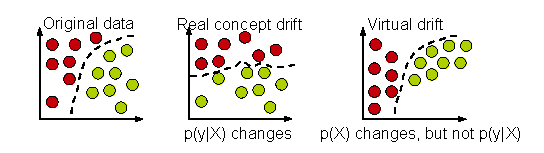
\includegraphics[height=0.15\textheight]{images_cropped/gama_survey_cd_fig1}
	\caption{Illustration from~\cite{gama2014survey} depicting real and virtual concept drift phenomena. Circles represent instances $x_i$, different colors - classes, dashed line is a decision boundary. }\label{fig:fig1_gama_survey_cd}
\end{figure}
\begin{figure}[htb!]
	\centering
	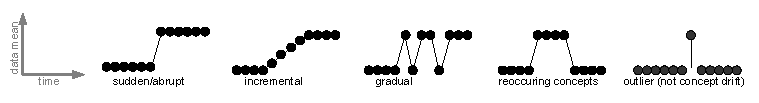
\includegraphics[width=0.9\textwidth]{images_cropped/gama_survey_cd_fig2}
  \caption{Changes between concepts can be gradual or abrupt~\cite{gama2014survey}}\label{fig:fig2_gama_survey_cd}
\end{figure}
\begin{figure}[htb!]
	\centering
	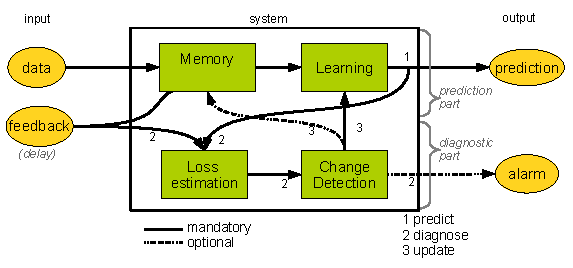
\includegraphics[width=0.9\textwidth]{images_cropped/gama_survey_cd_fig3}
  \caption{A generic schema for an online adaptive learning algorithm (from~\cite{gama2014survey})}\label{fig:fig3_gama_survey_cd}
\end{figure}


\section{The link between change detection and concept drift}

Concept drift and change detection in time series are closely related problems.
\textit{Concept} is a set of contiguous examples where the distribution is stationary.
In~\cite{gama2004learning} authors proposed a method to detect changes in the distribution of the training examples.
The drift detection method works by monitoring the online error-rate of a model.

The next paragraph is from~\cite{gama2004learning}.
Suppose a sequence of examples $(x_i, y_i)$.
For each example the model predicts $\hat y_i$ that can be True or False.
For a set of examples the error is a random variable from Bernoulli trials.
The probability of the number of errors for $n$ examples is given by the Binomial distribution.
Probability to observe False for an example $x_i$ is $p_i$ with the standard deviation $s_i=\sqrt{p_i(1-p_i)/i}$.
Statistical decision theory guarantees that while the class distribution of the examples is stationary, the error rate of the learning algorithm ($p_i$) will decrease when $i$ increases.
A significant increase in the error rate of the model implies a change in the class distribution.

SINE1~\cite{gama2004learning} artificial dataset.
In the first concept all points below the curve $y=sin(x)$ have label 1, and all points above have label 0.
After the concept change labelling is reversed.

Machine Learning models learn the relation between input data $x$ and target
variable $y$ by approximating a joint distribution $p(x,y)$.  Model performance
degrades when learned underlying data distribution changes.  Therefore concept
drift can be detected by monitoring change points in model's output performance
statistics.

\section{Example data: }
% https://sites.google.com/view/uspdsrepository
% pass: DMKD2018
~\cite{SouzaChallenges2020}


\section{Example: Arima concept drift example}
% https://otexts.com/fpp2/AR.html
Let's consider AR(1) process.
Autoregressive-integrated moving average (ARIMA)~\cite{box2015time} model models stationary processes when the process remains in equilibrium about a constant mean level.
Forecasts are usually needed over a period known as lead time $l$.

In the autoregressive model
the current value is expressed as 
let $\tilde{y}_t = y_t - \mu$
Equation~\ref{eq:ar_proc} is autoregressive (AR) process of order $p$
\begin{equation}\label{eq:ar_proc}
  y_{t} = c + \phi_{1}y_{t-1} + \phi_{2}y_{t-2} + \dots + \phi_{p}y_{t-p} + \varepsilon_{t},
\end{equation}
where $\varepsilon_{t}$ is a white noise. 
\begin{equation}\label{eq:ma_proc}
  y_{t} = c + \varepsilon_t + \theta_{1}\varepsilon_{t-1} + \theta_{2}\varepsilon_{t-2} + \dots + \theta_{q}\varepsilon_{t-q}
\end{equation}
for stationary processes constrains are~\cite{hyndman2018forecasting} 
\begin{itemize}
  \item for AR(1) $-1 < \phi_1 < 1$
  \item for AR(2) $-1 < \phi_2 < 1, \phi_1+\phi_2 <1, \phi_2-\phi_1 < 1$
\end{itemize}
\begin{figure}[!htb]
	\centering
	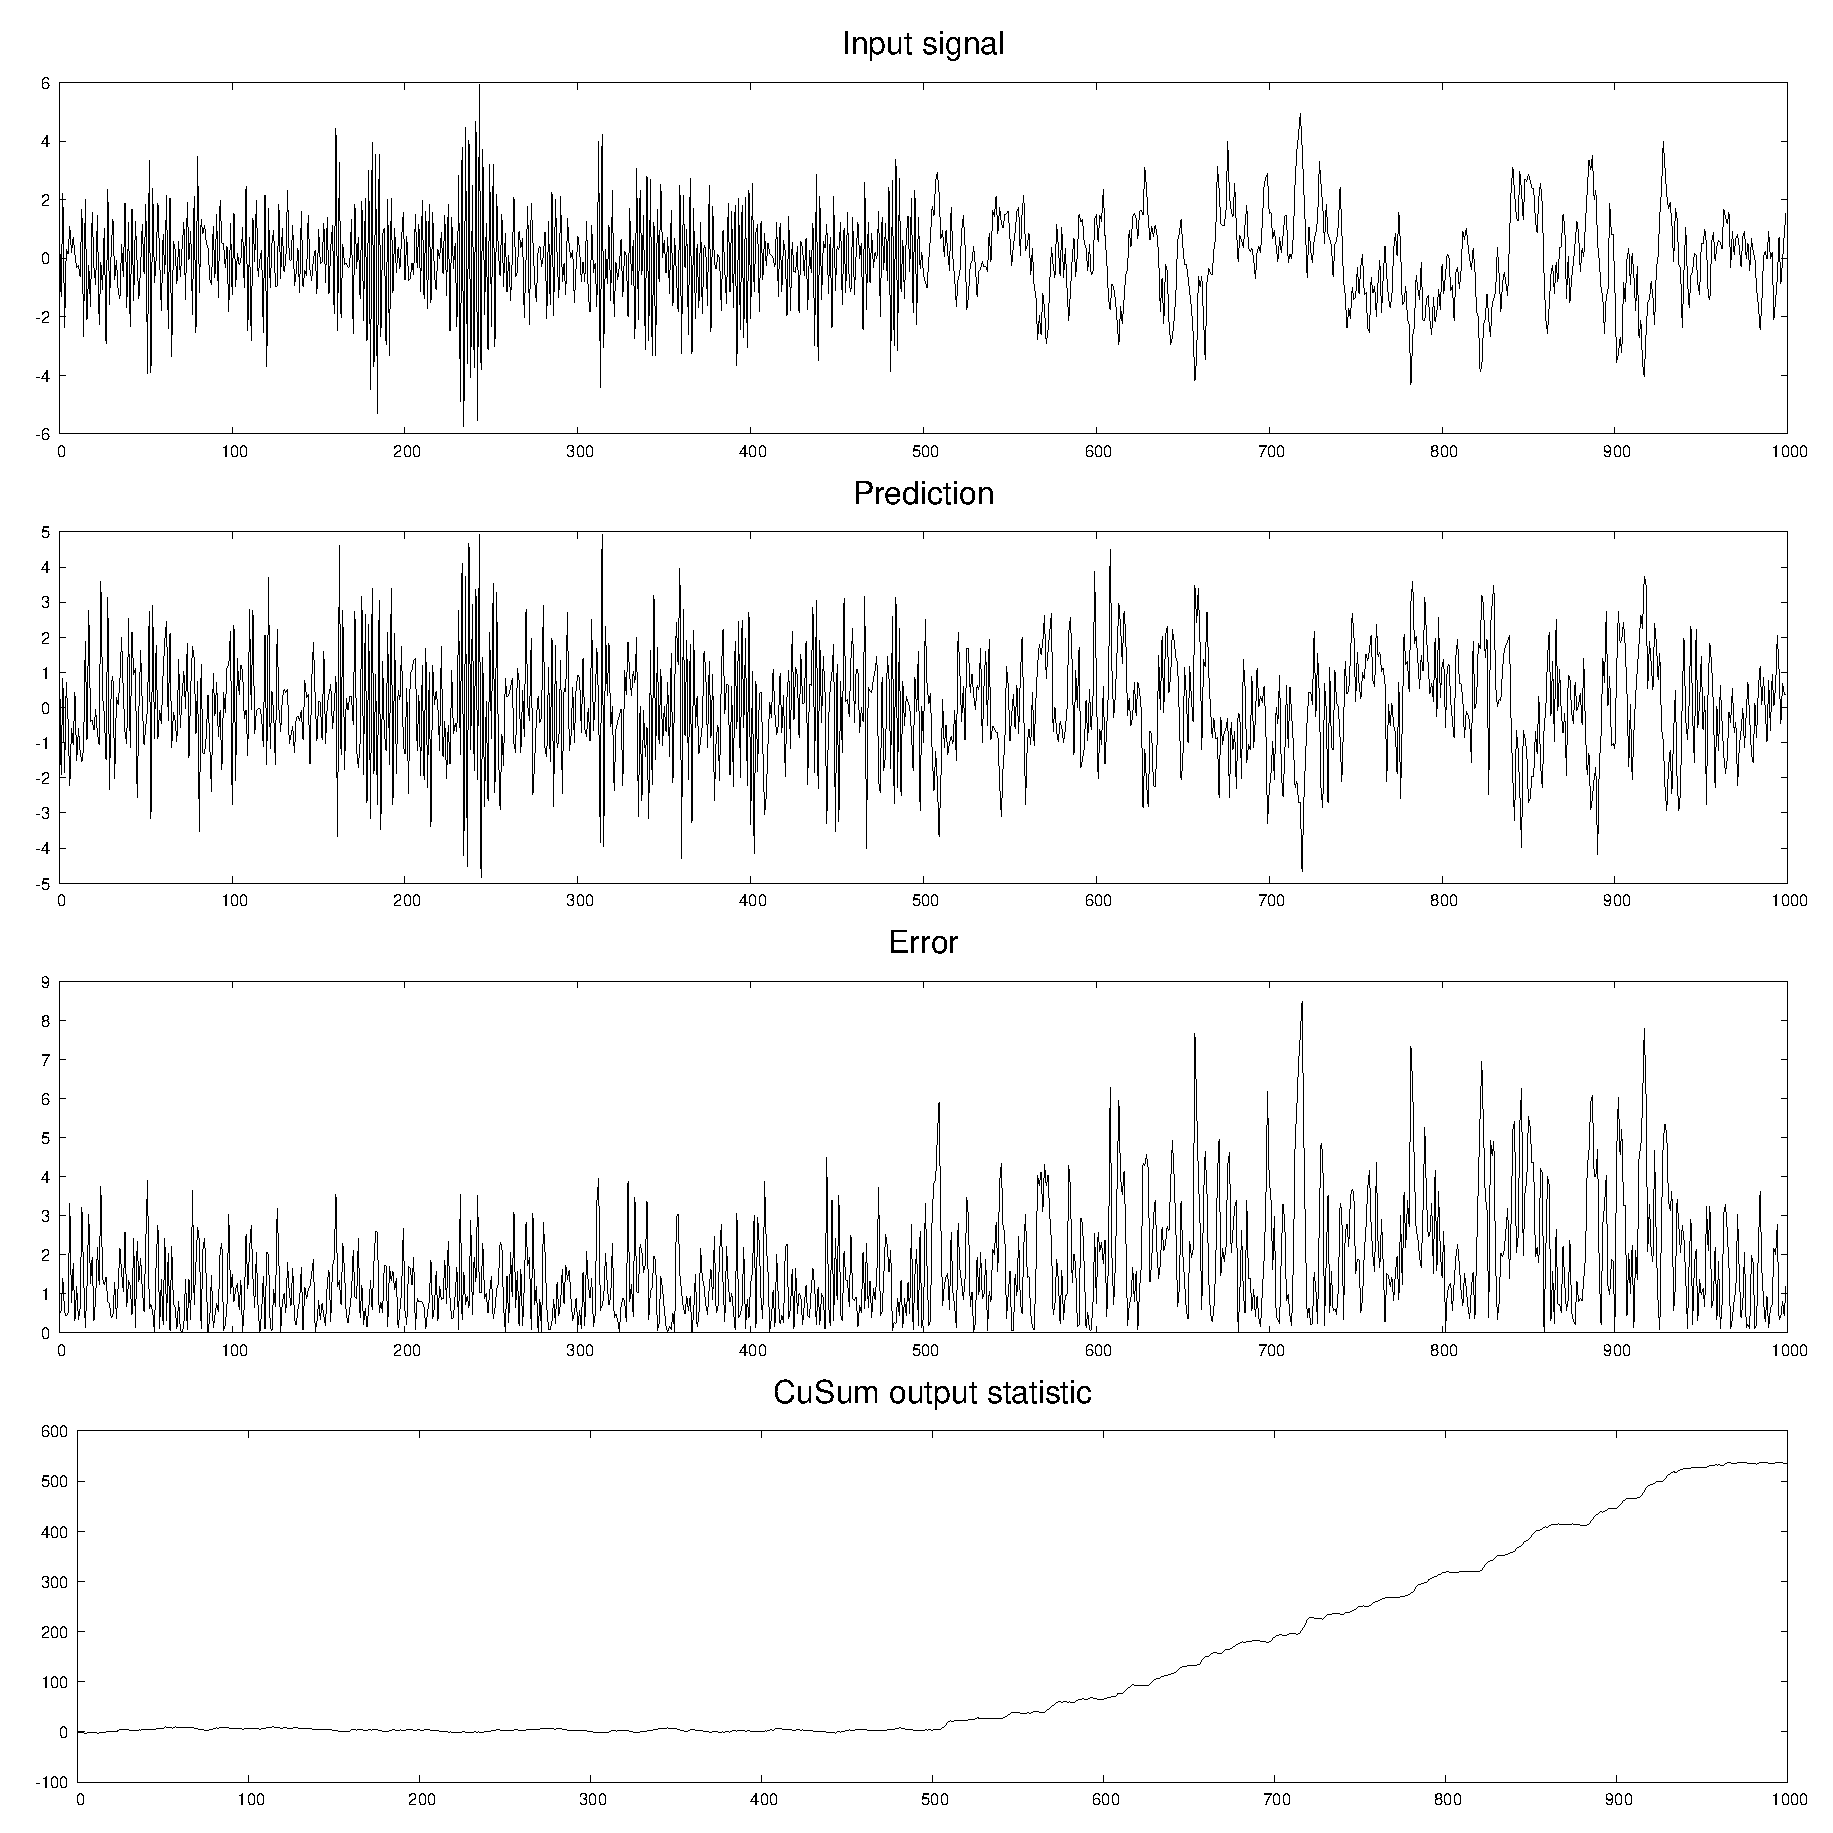
\includegraphics[width=0.9\textwidth]{images/arima_cd_example}
	\caption{Arima concept drift example.
		Two $AR(1) $ processes.
		First and second halfs of the signal is generated by the $AR(1)$ process
	}\label{fig:arima_cd_example}
\end{figure}
% \tilde{y}_t = \phi_1 \tilde{y}_{t-1} + \phi_2 \tilde{y}_{t-2} + \dots + \phi_p \tilde{y}_{t-p} + a_t
%where $a_t \sim \mathcal{N}(\mu, \sigma_a)$.


\section{Example: ELEC2}
The electricity market data set ELEC2~\cite{harries1999splice, gama2004learning} is widely used for testing adaptive learning techniques.
It should be noted however that it is not clear if there is a concept drift in the dataset~\cite{zliobaite2013good}. 
%https://www.openml.org/d/151
%Electricity is a widely used dataset described by M. Harries and analyzed by J. Gama (see papers below). This data was collected from the Australian New South Wales Electricity Market. In this market, prices are not fixed and are affected by demand and supply of the market. They are set every five minutes. Electricity transfers to/from the neighboring state of Victoria were done to alleviate fluctuations.
%
The dataset (originally named ELEC2) contains 45,312 instances dated from 7 May 1996 to 5 December 1998. 
Each example of the dataset refers to a period of 30 minutes, i.e. there are 48 instances for each time period of one day. 
Each example on the dataset has 5 fields, the day of week, the time stamp, the New South Wales electricity demand, the Victoria electricity demand, the scheduled electricity transfer between states and the class label. 
The class label identifies the change of the price (UP or DOWN) in New South Wales relative to a moving average of the last 24 hours (and removes the impact of longer term price trends). 
%
%The data was normalized by A. Bifet.
%
%### Attribute information  
%* Date: date between 7 May 1996 to 5 December 1998. Here normalized between 0 and 1
%* Day: day of the week (1-7)
%* Period: time of the measurement (1-48) in half hour intervals over 24 hours. Here normalized between 0 and 1
%* NSWprice: New South Wales electricity price, normalized between 0 and 1
%* NSWdemand: New South Wales electricity demand, normalized between 0 and 1
%* VICprice: Victoria electricity price, normalized between 0 and 1
%* VICdemand: Victoria electricity demand, normalized between 0 and 1
%* transfer: scheduled electricity transfer between both states, normalized between 0 and 1
\begin{figure}[!htb]
	\centering
	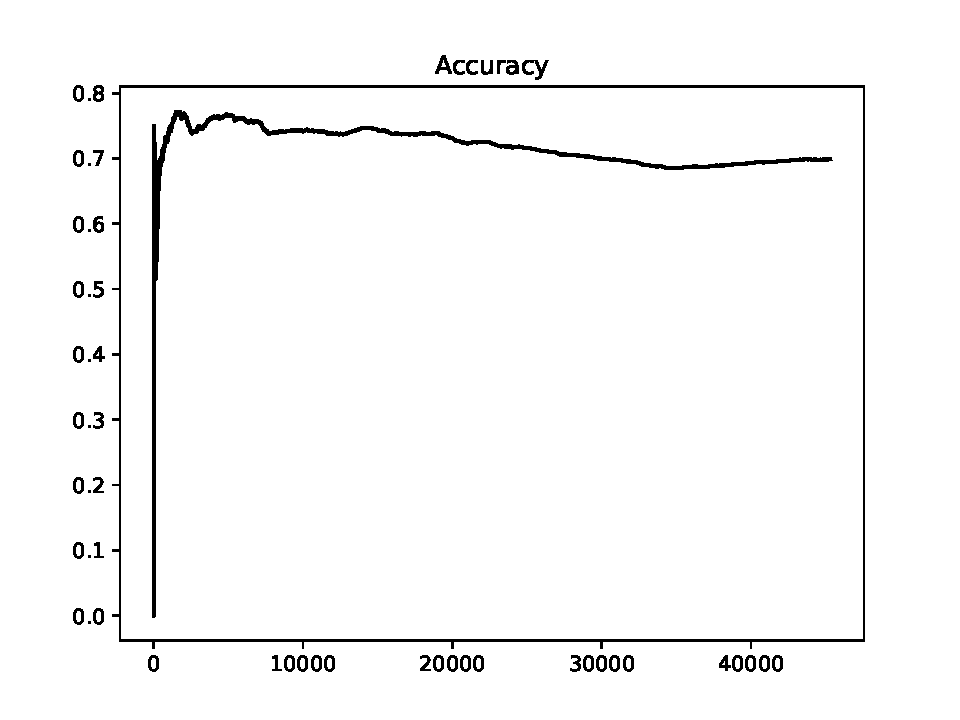
\includegraphics[width=0.9\textwidth]{images/cd_example_elec2.pdf}
	\caption{Elec2 dataset}\label{fig:elec2}
\end{figure}

\section{Example: SINE1}
\begin{figure}[!htb]
	\centering
	\includegraphics[width=0.9\textwidth]{images/cd_example_sine1}
	\caption{SINE1 artificial dataset. 
		Before concept drift (CD) all points above the curve $y=\sin(x)$ are classified as positive.
After CD - as negative.	
}\label{fig:sine1}
\end{figure}

\section{CFB boiler}
\begin{figure}[!htb]
	\centering
	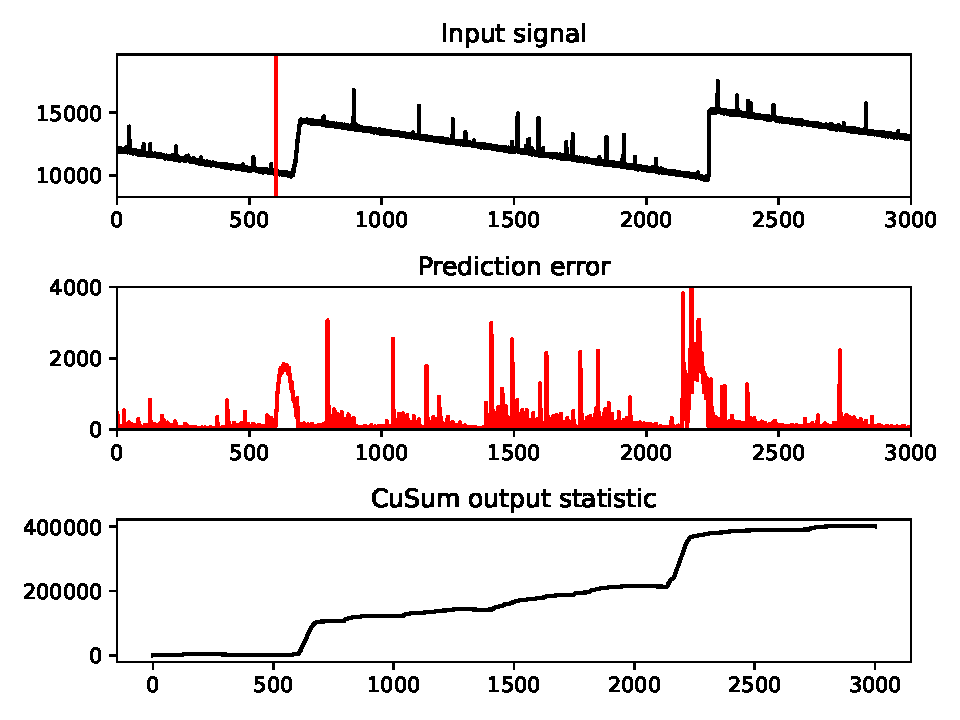
\includegraphics[width=0.9\textwidth]{images/boiler_fixed_train}
	\caption{CFB boiler signal.
Linear regression model is trained using first 600 observations (vertical red line).	
}\label{fig:boiler_fixed_train}
\end{figure}

\section{Change detection problem}

On-line change detection in time series data is an old practical problem with the roots in the problem of statistical quality control~\cite{basseville1993detection,NISTbook}.
Walter A. Shewhart invented control charts in 1924 while working on the problem of statistical quality control to improve reliability of telephone transmission systems. 
Quality control example: $X$ is a set of sensor readings and $y=good$ is a quality of the produced item. 
Offline and online. 
In offline learning all training data is available during training. 
In online learning the data is processed sequentially from data streams.
Model is being updated as more data arrives. 
Data evolve over time in dynamically changing environments.

\begin{figure}[!htb]
	\centering
	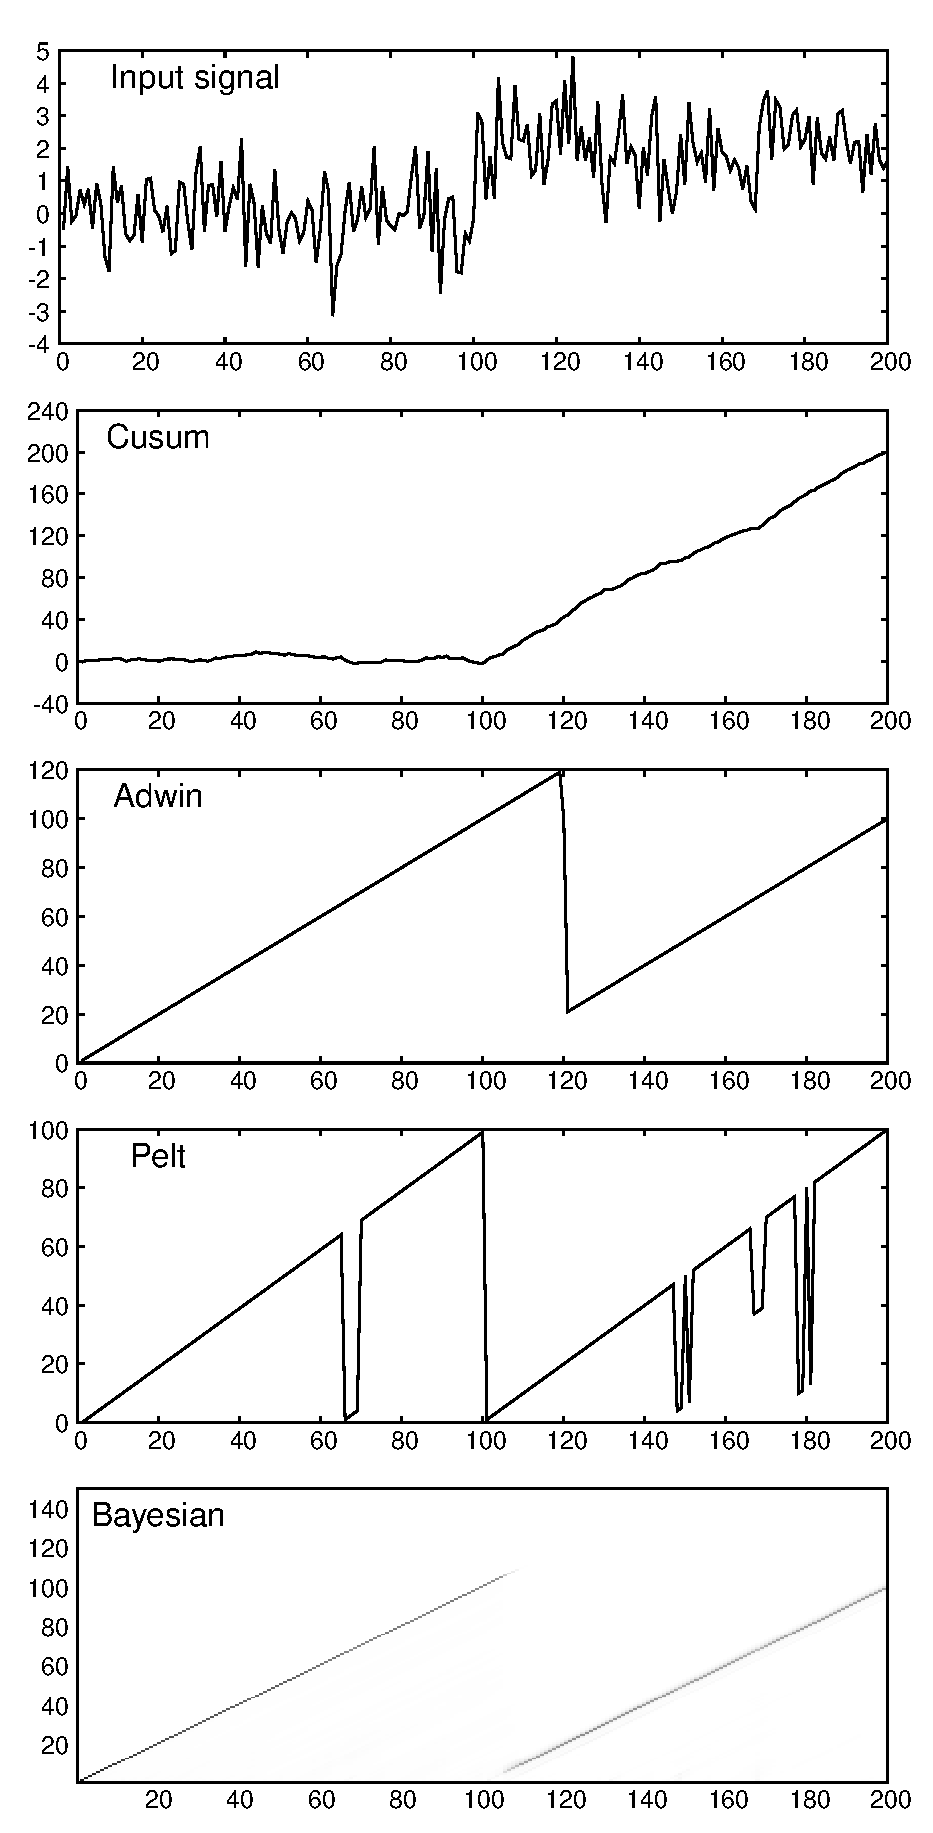
\includegraphics[height=0.9\textwidth]{images/detectors_output_stats}
	\caption{All}\label{fig:all_detectors_stats}
\end{figure}

\section{Detectors}
\subsection{Adwin}
Adwin was proposed in~\cite{bifet2007learning}.
Confidence value $\delta \in (0,1)$
Equation\ref{eq:adwin_ecut}.
\begin{equation}\label{eq:adwin_ecut}
	\epsilon_{\text{cut}} = \sqrt{\frac{2}{m} \cdot \sigma_W^2 \cdot \ln{\frac{2}{\delta^\prime}}} + \frac{2}{3m} \ln{\frac{2}{\delta^\prime}}
\end{equation}
Algorithm\ref{alg:adwin}
\begin{algorithm}[!h]
	\begin{algorithmic}[1]
		\Function{Adwin}{}
		\State Initialize window $W$
		\For{t $\in$ [1, n]}
		\State $W=W \cup x_t$\Comment{Add $x_t$ to the head of $W$} 
		\Repeat
		\State Drop elements from the tail of $W$
		\Until{$|\mu_{W_0} - \mu_{W_1}|\geq \epsilon_{\text{cut}}$ holds for every split of $W=W_0\cdot W_1$}
		\EndFor
		\EndFunction
	\end{algorithmic}
	\caption{Adwin pseudocode \cite{bifet2007learning}}\label{alg:adwin}
\end{algorithm}
\begin{figure}[!htb]
	\centering
	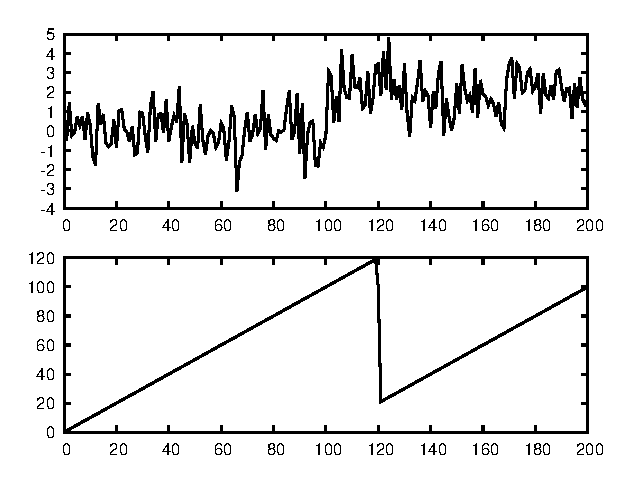
\includegraphics[width=0.9\textwidth]{images/example_output_adwin.eps}
	\caption{ADWIN}\label{fig:adwin_output_example}
\end{figure}

\subsection{Pelt method}

Offline detector used in online settings in ~\cite{marrero2013aclac}.
~\cite{killick2012optimal}
Pelt method is based on a common approach of  minimising a cost function over possible numbers and locations of change points.
Pelt is based on~\cite{jackson2005algorithm}, but involves a pruning step reducing the computational cost but not affecting exactness of the resulting segmentation.
Dynamic programming~\cite{bellman1966dynamic}.

Time interval $I$.
Ordered sequence of data $y_{1:n}=(x_1,\dots,y_n)$.
A partition $P$ of an interval $I$ is a set of blocks is defined  by change points $\tau_{1:m}=(\tau_1, \dots, \tau_m)$.
Each change point is an integer between 1 and $n-1$.
We define $\tau_0=0$ and $\tau_{m+1}=n$.
$m$ change points split the data into $m+1$ segments, $i$-th segment is $y_{\tau_{i-1} : \tau_i}$.
For example, if there is one changepoint $\tau_1$ the segments are $B_1=y_{\tau_0:\tau_1}$ and $B_2=y_{\tau_1:\tau_2}$ where $\tau_2 \equiv n$.
The goal is to find an optimal partition by minimising the cost function defined by Equation\ref{eq:cost_function}
\begin{equation}\label{eq:cost_function}
	\sum_{i=1}^{m+1} [ C(B_i) ] + \beta f(m),\: \text{where } B_i \equiv y_{\tau_{i-1} : \tau_i}
\end{equation}
where $\beta f(m)$ is a regularization term to prevent overfitting.
Commonly used cost functions are twice the negative log likelihood~\cite{guyon1999underfitting,chen2011parametric},
quadratic loss and cumulative sums~\cite{inclan1994use, rigaill2010pruned}.
The most common choices for the regularization term are usually $\beta f(m) = \beta m$.
Examples are Akaike's Information Criterion (AIC\cite{akaike1974new}) $\beta=2p$ and Schwartz Information Criterion (BIC\cite{schwarz1978estimating}) ($\beta = p \log{n}$) where $p$ is the number of additional parameters introduced by adding a new changepoint.
Dynamic programming optimal segmentation is based on the next principle of optimality
\begin{theorem}
Let $P^{\text{max}}$ be an optimal optimal partition of $I$
\end{theorem}

\begin{algorithm}[!h]
	\begin{algorithmic}[1]
		\Function{pelt}{$Y$, $\sigma$, $C(s,t)$}
		\State n = length($Y$)
		\State $F$ = zeros(n)\Comment{Optimal segmentation costs till $t$}
		\State $F[0] = - \log(n)$
		\State previous\_changes\_opt = zeros[n]\Comment{Optimal previous change location}
		\For{t $\in$ [2, n]}
		\State previous\_changes\_possible = $1,\dots,t-1$
		\State i = 0
		\For{s $\in$ previous\_changes\_possible}
		\State i += 1
		\State segmentation\_costs[i] = $C(s, t)$
		\EndFor
		\State costs = $F[\text{previous\_changes\_possible}]$ + segmentation\_costs + $\log(n)$
		\State $F[t+1] = min(\text{costs})$
		\State $\text{previous\_changes\_opt}[t] = \text{previous\_changes\_possible}[argmin(\text{costs})]$
		\EndFor
		\State detections = $\text{fn\_extract\_detections(previous\_changes\_opt)}$
		\EndFunction
	\end{algorithmic}
	\caption{Pelt algorithm}\label{alg:pelt}
\end{algorithm}
\begin{figure}[!htb]
	\centering
	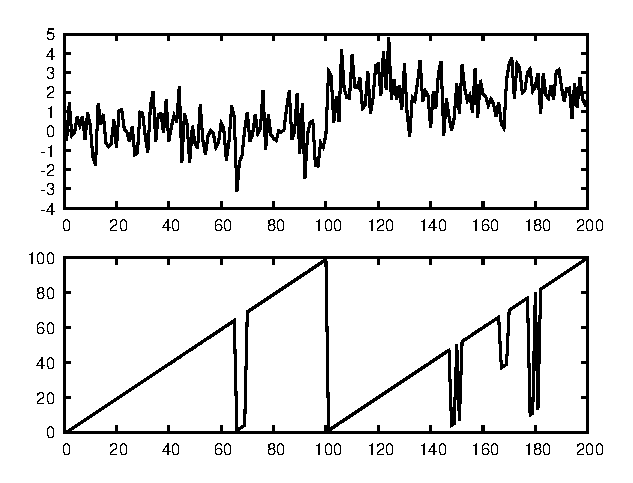
\includegraphics[width=0.9\textwidth]{images/example_output_pelt.eps}
	\caption{PELT}\label{fig:pelt_output_example}
\end{figure}

\subsection{Bayesian detector}

\cite{adams2007bayesian}
BD detector works by recursively estimating posterior probability distribution $P(r_t | \pmb{x}_{1:t}, \theta)$ of the \textit{run length} variable $r_t$ which is a time since the last changepoint.
Changepoint is an event when
\begin{equation}
	\operatorname*{arg\,max}_{r_t} P(r_t | \pmb{x}_{1:t}, \theta) = 0
\end{equation}
%$r_t = 0$
Every time a new measurement $x_t$ is observed the \textit{posterior} distribution is recalculated using the Bayes` theorem to update parameters of the distributions used to model data
\[
(r_t | \pmb{x}_{1:t}) = \frac{P(r_t, \pmb{x}_{1:t})}{P(\pmb{x}_{1:t})}
\]
and the law of total probability
%$P(x) = \sum_{y} P(x|y) p(y)$
\begin{equation}
	P(r_t|\:\LargeCdot) = \sum_{r_{t-1}} P(r_{t} | \: r_{t-1},\:\LargeCdot) \: P(r_{t-1}|\:\LargeCdot)
\end{equation}
to take into account values from all the runs in the past.
The \textit{prior} probability of the change $P(r_t=0|t)$ in BD detector is specified using the constant-value hazard rate $h$ which is a prior probability to observe a change and which is supposed to be known before the change detection process starts.
\begin{figure}[!htb]
	\centering
	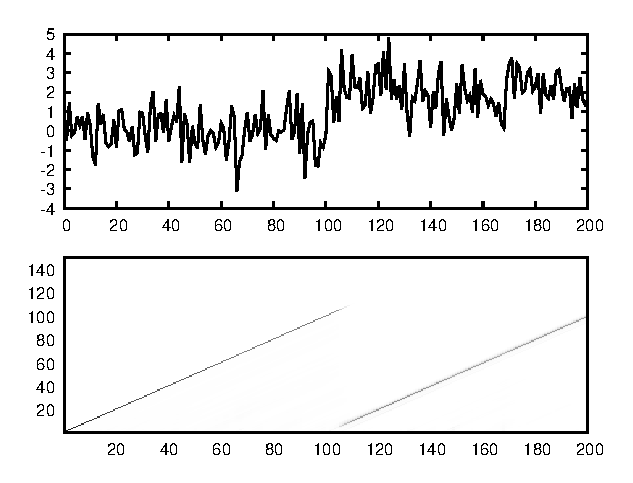
\includegraphics[width=0.9\textwidth]{images/example_output_bayes.eps}
	\caption{Bayes}\label{fig:bayes_output_example}
\end{figure}

\subsection{CUSUM detector}

In this section, we describe the CuSum~\cite{Page1954} detector and its output statistic properties important for measuring performance metrics in static and dynamic settings.
Changes in the stream of measurements reflect dynamics of observed phenomenon happening in time.
Therefore, strictly speaking, any change is a gradual process.
In this paper, for simplicity, we refer to change points and to detections as individual time moments as if change would have happen instantly. If change is gradual and spans time interval then it can be reduced to a single time moment by considering the start or end of the change event~\footnote{Gradual change may become represented as an abrupt change in the time series also due to the sampling rate of measurements}.
Change points in the signal are characterized by the time moment when they happened and by the corresponding mean shift value in the signal.
\begin{definition}
	Change point is a time moment $t^c$ when statistical properties of the data stream change significantly accordingly to a predefined criteria.
\end{definition}
\begin{definition}
	Detection is a time moment $t^d$ when a detector alarms a change.
\end{definition}
For example, if $x_i \sim \mathbb{N}(\mu_1, \sigma)$ for $i < k$ and $x_i \sim \mathbb{N}(\mu_2, \sigma)$ for $i \geq k$,
then we say that a change point occurred at time moment $t_k$, i.e. $t^{\text{c}}_{k} \equiv t_k$.
In general, detection can usually be alarmed before or after a change point.
If $t^{\text{d}}_k > t^{\text{c}}_k$, then change is detected with the delay $t^{\text{d}}_k - t^{\text{c}}_k$.
%TOMMI: Can we give definition like below? I.e. to say that ALL too-early alarms are false alarms?
If $t^{\text{d}}_k < t^{\text{c}}_k$ then detection $t^{\text{d}}_k$ is a false alarm (FA).

As an input, CuSum detector receives time series of observations~\ref{eq:input_ts} usually taken at constant sampling rate.
\begin{equation}\label{eq:input_ts}
	(x_i)_{i=1}^{N} \equiv (x_1, x_2, \dots, x_N)
\end{equation}
taken at corresponding time moments $(t_i)_{i=1}^N$.
Observations and time moments are enumerated by index $i$ mapping $t_i$ to observations $x_i$ and vice versa.
CuSum works through a sequential calculation of the output statistic as follows
% Cusum rule: https://www.itl.nist.gov/div898/handbook/pmc/section3/pmc323.htm
\begin{align}
	S_0 &= 0 \nonumber \\
	S_{n} &= \max (0, S_{n-1} + x_n - \mu_0 - k )\label{eq:cusum_scheme}.
\end{align}
% Detections are alarmed at time moments when Cusum's output statistic exceeds a threshold value $h$.
Detections are alarmed at time moments when $S_{t+1} > h$, i.e. when output statistic exceeds a threshold value $h$.
In \eqref{eq:cusum_scheme}, $\mu_0$ is the estimate of the in-control state signals' mean value.
The parameter $k$ is called allowance value and it depends on the level of mean shift $\delta=\mu_2-\mu_1$ that we aim to detect.

\begin{algorithm}
	% class Detector
	\begin{algorithmic}[1]
		%\Function{CusumSingle}{$X$, $h$, $\text{PCCF}$}\Comment{Single changepoint detection}
		%\State n=length($X$)
		%\State stat=zeros(n)
		%\State stat[0]=X[0] - $\mu_0$
		%\For{t $\in$ [1,n]}
		%\State stat[t] = stat[t-1]+X[t]-$\mu_0$
		%\If{(not PCCF) or (PCCF and WithinRoi()) }
		%\If{$|stat[t]| > h$}
		%\State \Return (t, stat) \Comment{Alarm CDE}
		%\EndIf
		%\EndIf
		%\EndFor
		%\State \Return (nan, stat)\Comment{Return missing value for CDE}
		%\EndFunction  
		%\\
		\Function{CusumMutli}{$X$, $h$, $\text{PCCF}$}\Comment{Sequential/multi- changepoint detection}
		\State n = length(Signal)
		\State detections = [ ]
		\For{t $\in$ [1,n]}
		%\While{$t <n$}
		\State UpdateMu(Signal[t])
		\State UpdateCusumStatistic()
		\If{PCCF and EnteredRoi()}
		\State NextRoiIndex $\mathrel{{+}{=}} 1$
		\EndIf
		%\Comment{If we don't use Pccf or we use Pccf and we are inside ROI}
		\If{(not PCCF) or (PCCF and WithinRoi()) }
		\If{$|stat[t]| > h$}
		\State detections.append(t) \Comment{Collect CDEs}
		\State ResetDetector()
		\EndIf
		\EndIf
		%\State t $\mathrel{{+}{=}} 1$
		%\EndWhile
		\EndFor
		\If{len(detections) == 0} \Comment{In case of detecting single change point}
		\State delay = NaN \Comment{Return detection delay NaN if no detection is alarmed}
		\EndIf
		\State \Return detections 
		\EndFunction
		\\
		\Function{UpdateMu}{}\Comment{Running mean value after each CDE}
		\State $\mu_{t}=\frac{k-1}{k} \mu_{t-1} + \frac{x}{k}  $
		\EndFunction
		\\
		\Function{UpdateCusumStatistic}{}\Comment{Update CUSUM statistic}
		\State $\delta = x_t - \mu_t$
		\State $stat[0] = \delta$
		\State $stat[t] = stat[t-1] + \delta \: \forall \: t >0$
		\EndFunction
		\\
		\Function{ResetDetector}{}\Comment{Re-initialize detector after each CDE}
		\State $\mu_t=0$
		\State k=1
		\State $stat[t]=x_t$
		\EndFunction
	\end{algorithmic}
	\caption{Cusum for single and multiple change points detection.}\label{alg:method_code}
\end{algorithm}


\begin{figure}[!htb]
	\centering
	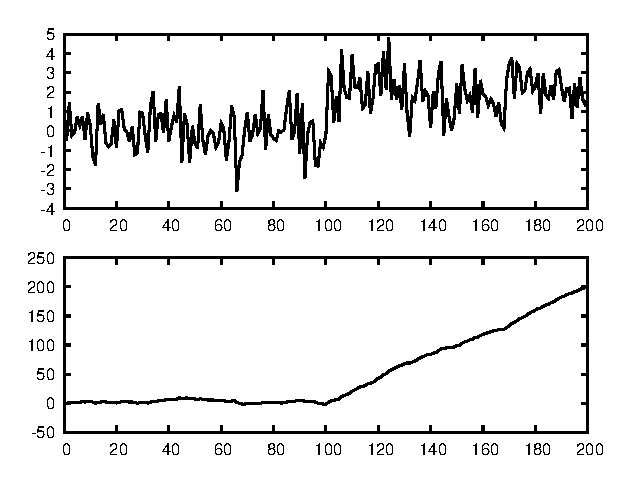
\includegraphics[width=0.7\textwidth]{images/example_output_cusum.eps}
	\caption{CuSum}\label{fig:cusum_output_example}
\end{figure}

\subsection{ARL}

The key performance metric of the CuSum detector is the Average Run Length (ARL), which refers to the expected number of observations before an action is taken, i.e., before the detection is alarmed~\cite{Page1954}.
ARL refers to the FA rate before the change and to the detection delay after the change point.
When the process is in-control, the $ARL_{\delta}$ refers to a FA rate, whereas when the change has happened it refers to the detection delay.
% ARL approximation in Equation~\ref{eq:arl_approximation} is given by~\cite{siegmund2013sequential}.
However, ARL is hard to estimate analytically.
As reported in~\cite{plasse2021streaming}, one of the simplest ARL approximations is given in~\cite{siegmund2013sequential} in a form of the following equation %Equation~\ref{eq:arl_approximation}
\begin{equation}\label{eq:arl_approximation}
	\text{ARL}_{\delta} = \frac{\exp(-2(\delta-k)h') + 2(\delta - k)h' -1}{2 (\delta - k)^2}
\end{equation}
%Here, $\delta=\mu_2-\mu_1$ is the mean shift we aim to detect and
for $h' = h+1.166$.
Figure~\ref{fig:arl} depicts ARL behavior against $\delta$ (left plot) and versus threshold $h$ (right plot).
It is easy to see how ARL refers to both the FA rate and to the detection delay at the same time.
More precisely, smaller values of $\delta$ correspond to fluctuations in the signal and to the larger ARL values, whereas
larger values of $\delta$ indicate change points to be detected.
Not surprisingly, ARL decreases fast when $\delta$ is increased.
It also can be seen that by changeing $\delta$ we increase or decrease ARL value.
We will use this fact later in the experimental part when performing simulations to measure the detection delay by varying ARL values (by changing $\mu_2-\mu_1 \equiv \delta$) for static and dynamic detectors.
%
\begin{figure}[!htb]
	\centering
	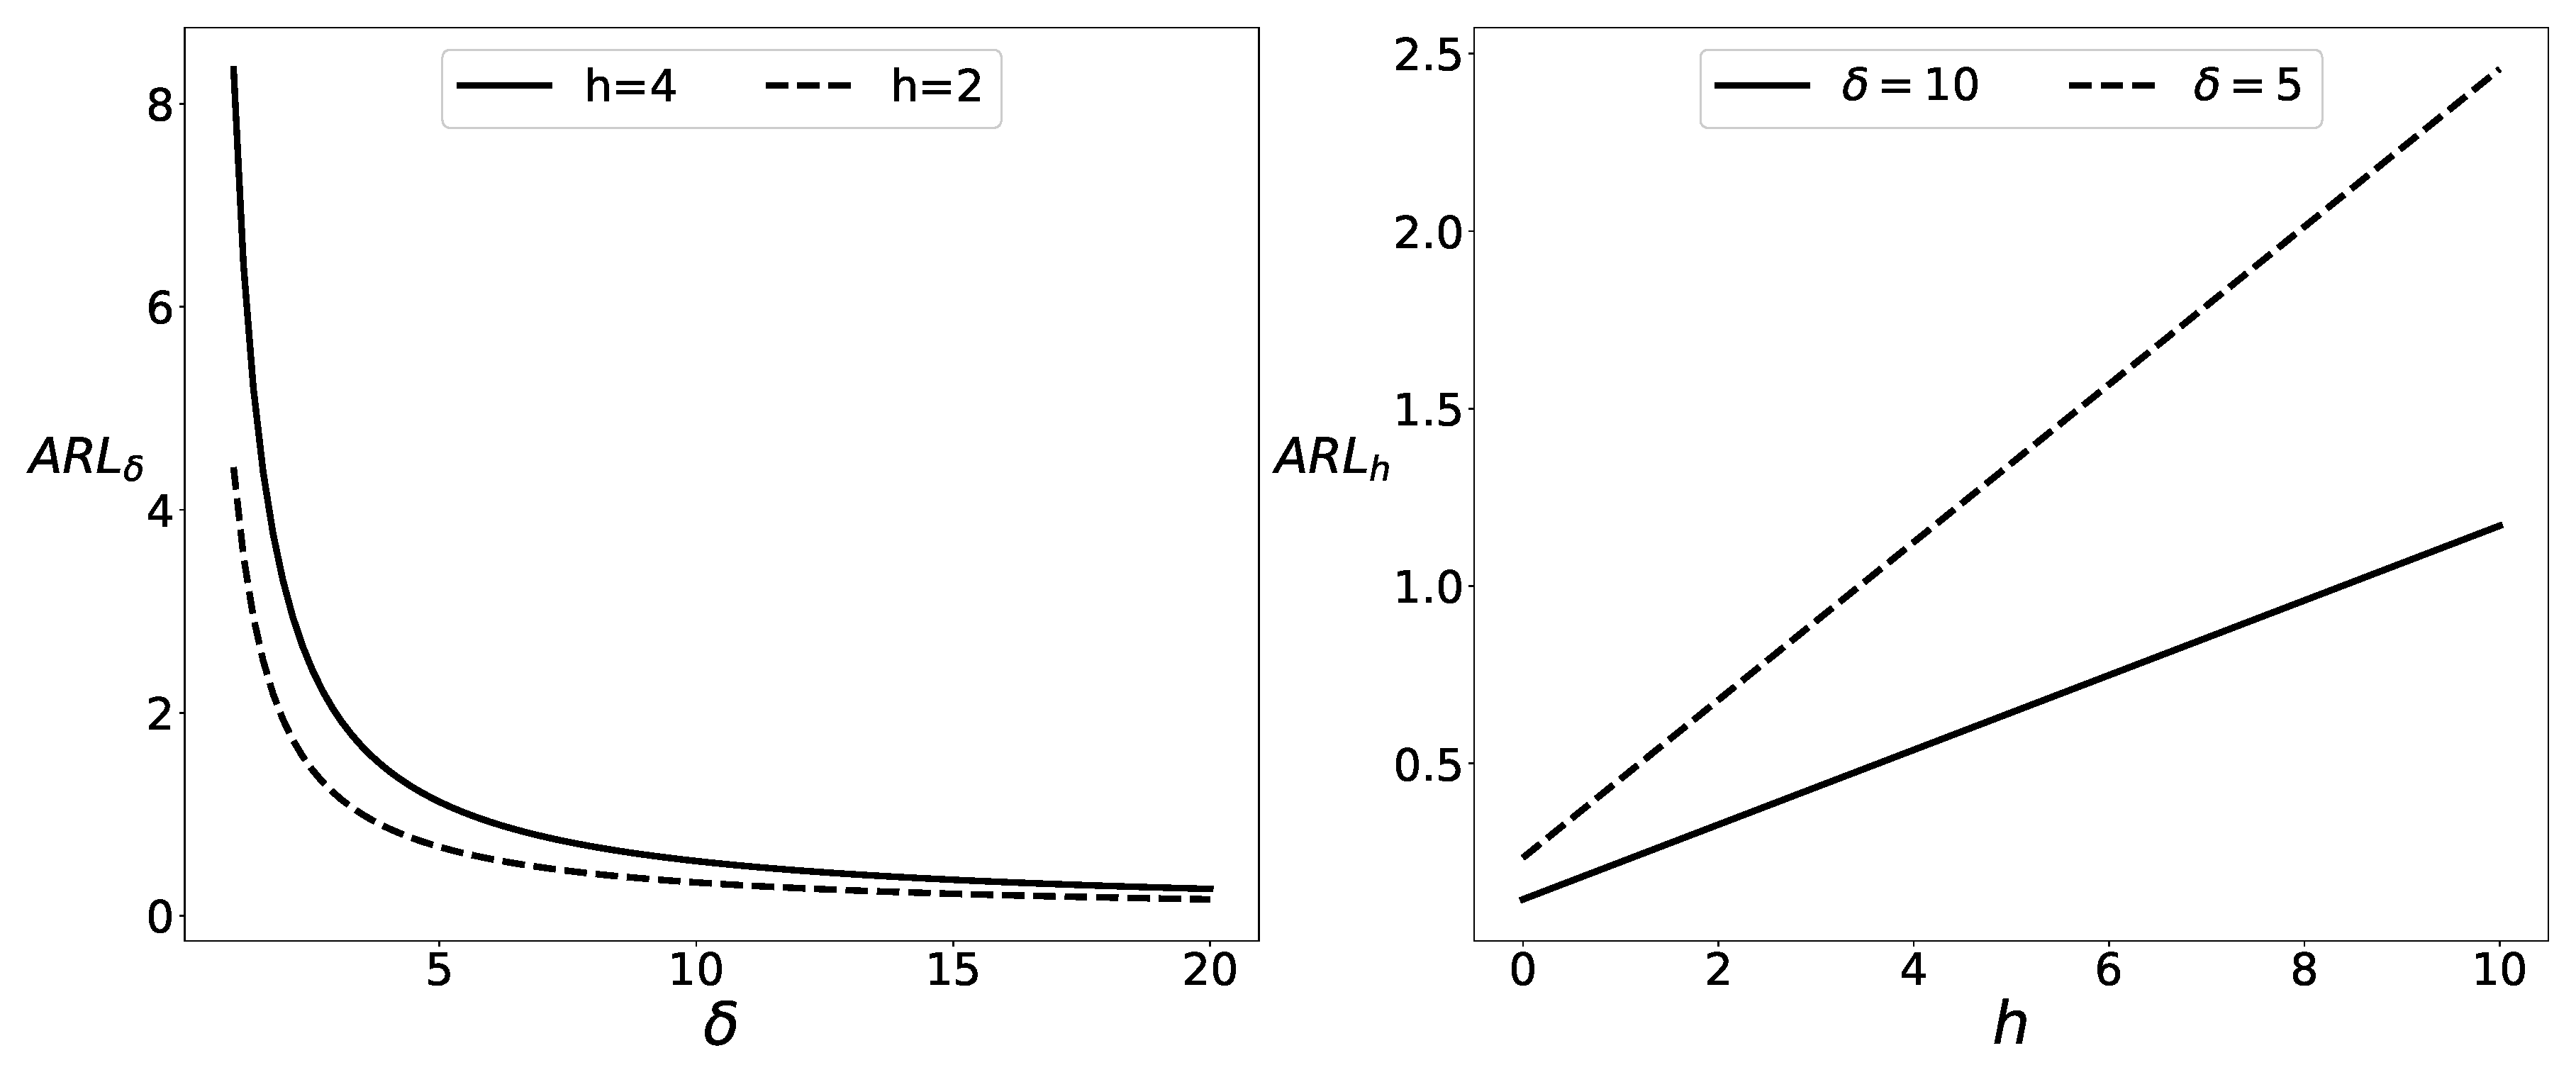
\includegraphics[width=0.9\textwidth]{images_ecmplpkdd/arl.eps}
	\caption{
    The left plot depicts ARL as a function of $\delta = \mu_2-\mu_1$ for two fixed threshold values $h$. The right plot depicts ARL as a function of the threshold value $h$ for two fixed $\delta$ values (Equation~\ref{eq:arl_approximation}).
    Both plots demonstrate that smaller ARL values (and therefore detection delays) correspond to smaller $h$ values. It is obvious for the right plot, on the left plot this fact is depicted by the dashed line for $h=2$ being lower than the solid line for $h=4$.
    %
    Smaller $\delta$ corresponds to the fluctuations in the time series causing false alarms, larger $\delta$ correspond to changes in the level shift which are subject for detection.
    When threshold $h$ is adjusted to smaller values ARL for all $\delta$ values gets smaller (left plot), therefore detection delay is decreased but probability of FA is increased.
    %Left plot depicts that ARL values for the whole range of $\delta$ values are decreased including smaller $\delta$ values corresponding to FA events,i.e.\ average runs between false alarms are also decreased along with the detection delay.
    %
    % Our hypothesis which we investigate experimentally is that by using smaller values of $h$ within prediction intervals and by disregarding detections outside of them we can decrease detection delay and the total number of false alarms despite decreased average runs between them.
}\label{fig:arl}
\end{figure}
%\begin{figure}[!htb]
%	\centering
%	\includegraphics[width=0.7\textwidth]{images/arl3d.eps}
%	\caption{}
%\end{figure}
\begin{figure}[!htb]
% GNUPLOT: LaTeX picture with Postscript
\begingroup
  \makeatletter
  \providecommand\color[2][]{%
    \GenericError{(gnuplot) \space\space\space\@spaces}{%
      Package color not loaded in conjunction with
      terminal option `colourtext'%
    }{See the gnuplot documentation for explanation.%
    }{Either use 'blacktext' in gnuplot or load the package
      color.sty in LaTeX.}%
    \renewcommand\color[2][]{}%
  }%
  \providecommand\includegraphics[2][]{%
    \GenericError{(gnuplot) \space\space\space\@spaces}{%
      Package graphicx or graphics not loaded%
    }{See the gnuplot documentation for explanation.%
    }{The gnuplot epslatex terminal needs graphicx.sty or graphics.sty.}%
    \renewcommand\includegraphics[2][]{}%
  }%
  \providecommand\rotatebox[2]{#2}%
  \@ifundefined{ifGPcolor}{%
    \newif\ifGPcolor
    \GPcolorfalse
  }{}%
  \@ifundefined{ifGPblacktext}{%
    \newif\ifGPblacktext
    \GPblacktexttrue
  }{}%
  % define a \g@addto@macro without @ in the name:
  \let\gplgaddtomacro\g@addto@macro
  % define empty templates for all commands taking text:
  \gdef\gplbacktext{}%
  \gdef\gplfronttext{}%
  \makeatother
  \ifGPblacktext
    % no textcolor at all
    \def\colorrgb#1{}%
    \def\colorgray#1{}%
  \else
    % gray or color?
    \ifGPcolor
      \def\colorrgb#1{\color[rgb]{#1}}%
      \def\colorgray#1{\color[gray]{#1}}%
      \expandafter\def\csname LTw\endcsname{\color{white}}%
      \expandafter\def\csname LTb\endcsname{\color{black}}%
      \expandafter\def\csname LTa\endcsname{\color{black}}%
      \expandafter\def\csname LT0\endcsname{\color[rgb]{1,0,0}}%
      \expandafter\def\csname LT1\endcsname{\color[rgb]{0,1,0}}%
      \expandafter\def\csname LT2\endcsname{\color[rgb]{0,0,1}}%
      \expandafter\def\csname LT3\endcsname{\color[rgb]{1,0,1}}%
      \expandafter\def\csname LT4\endcsname{\color[rgb]{0,1,1}}%
      \expandafter\def\csname LT5\endcsname{\color[rgb]{1,1,0}}%
      \expandafter\def\csname LT6\endcsname{\color[rgb]{0,0,0}}%
      \expandafter\def\csname LT7\endcsname{\color[rgb]{1,0.3,0}}%
      \expandafter\def\csname LT8\endcsname{\color[rgb]{0.5,0.5,0.5}}%
    \else
      % gray
      \def\colorrgb#1{\color{black}}%
      \def\colorgray#1{\color[gray]{#1}}%
      \expandafter\def\csname LTw\endcsname{\color{white}}%
      \expandafter\def\csname LTb\endcsname{\color{black}}%
      \expandafter\def\csname LTa\endcsname{\color{black}}%
      \expandafter\def\csname LT0\endcsname{\color{black}}%
      \expandafter\def\csname LT1\endcsname{\color{black}}%
      \expandafter\def\csname LT2\endcsname{\color{black}}%
      \expandafter\def\csname LT3\endcsname{\color{black}}%
      \expandafter\def\csname LT4\endcsname{\color{black}}%
      \expandafter\def\csname LT5\endcsname{\color{black}}%
      \expandafter\def\csname LT6\endcsname{\color{black}}%
      \expandafter\def\csname LT7\endcsname{\color{black}}%
      \expandafter\def\csname LT8\endcsname{\color{black}}%
    \fi
  \fi
    \setlength{\unitlength}{0.0500bp}%
    \ifx\gptboxheight\undefined%
      \newlength{\gptboxheight}%
      \newlength{\gptboxwidth}%
      \newsavebox{\gptboxtext}%
    \fi%
    \setlength{\fboxrule}{0.5pt}%
    \setlength{\fboxsep}{1pt}%
\begin{picture}(8640.00,8640.00)%
    \gplgaddtomacro\gplbacktext{%
      \csname LTb\endcsname%%
      \put(1055,1901){\makebox(0,0){\strut{}$0$}}%
      \put(1670,1752){\makebox(0,0){\strut{}$0.5$}}%
      \put(2285,1604){\makebox(0,0){\strut{}$1$}}%
      \put(2901,1455){\makebox(0,0){\strut{}$1.5$}}%
      \put(3516,1307){\makebox(0,0){\strut{}$2$}}%
      \put(4131,1158){\makebox(0,0){\strut{}$2.5$}}%
      \put(4746,1010){\makebox(0,0){\strut{}$3$}}%
      \put(5197,1245){\makebox(0,0){\strut{}$0$}}%
      \put(5733,1491){\makebox(0,0){\strut{}$2$}}%
      \put(6269,1736){\makebox(0,0){\strut{}$4$}}%
      \put(6806,1981){\makebox(0,0){\strut{}$6$}}%
      \put(7342,2226){\makebox(0,0){\strut{}$8$}}%
      \put(7879,2472){\makebox(0,0){\strut{}$10$}}%
      \put(1008,3569){\makebox(0,0)[r]{\strut{}$0$}}%
      \put(1008,3965){\makebox(0,0)[r]{\strut{}$50$}}%
      \put(1008,4362){\makebox(0,0)[r]{\strut{}$100$}}%
      \put(1008,4758){\makebox(0,0)[r]{\strut{}$150$}}%
      \put(1008,5154){\makebox(0,0)[r]{\strut{}$200$}}%
      \put(1008,5551){\makebox(0,0)[r]{\strut{}$250$}}%
      \put(1008,5948){\makebox(0,0)[r]{\strut{}$300$}}%
      \put(1008,6345){\makebox(0,0)[r]{\strut{}$350$}}%
    }%
    \gplgaddtomacro\gplfronttext{%
      \csname LTb\endcsname%%
      \put(2604,2003){\makebox(0,0){\strut{}${\delta}$}}%
      \put(5891,1997){\makebox(0,0){\strut{}$h$}}%
      \put(210,4956){\makebox(0,0){\strut{}ARL}}%
    }%
    \gplbacktext
    \put(0,0){\includegraphics[width={432.00bp},height={432.00bp}]{/home/ms314/1/thesis/images/arl3d}}%
    \gplfronttext
  \end{picture}%
\endgroup

\caption{ARL 3D}\label{fig:arl3d}
\end{figure}


\chapter{Recurrency}

Adaptive learning in concept drift.
Predictability of events in the data stream.
~\cite{feller2008introduction}
Sums of independent random variables.
Recurrency is a form of predictability.

\section{Feller}
The basic theory is as follows~\cite{feller2008introduction}.
In a sequence of Bernoulli trials the waiting time up to the first event gas a geometric distribution.
After the first event the process starts anew, and the number of trials between $n$ and $n+1$ th events has the same geometric distribution.
\begin{definition}
	Let $a_1, a_2, \dots, $ be a sequence of real numbers. If 
	\begin{equation}
		A(s) = a_0 + a_1 s + a_2 s^2 + \dots 
	\end{equation}
    converges in some interval $-s_0 < s < s_0 $ , then $A(s)$ is called the generarating function of the sequence $\{a_j\}$. 
\end{definition}

From\cite{wasserman2013all}
\begin{definition}
	The moment generating function MGF, or Laplace transform, of $X$ is defined by
	\begin{equation}
		\psi_X = \mathbb{E}(e^{tX}) = \int e^{tX} dF(x) 
	\end{equation}
where $t$ varies over the real numbers.
\end{definition}

\section{Inter-arrival times modeling}
Basic theory.
\begin{definition}
	A function $\mathbb{P}$ that assigns a real number $\mathbb{P}(A)$ to each event $A$ is a probability distribution if \\
	Axiom 1: $\mathbb{P}(A) \geq 0$ for every $A$\\
	Axiom 2: $\mathbb{P}(\Omega) = 1$\\
	Axiom 3: If $A_1, A_2, \dots $ are disjoint then 
	\begin{equation}
		\mathbb{P} \Big( \bigcup\limits_{i=1}^{\infty} A_i  \Big) = \sum_{i=1}^{\infty} \mathbb{P}(A_i)
	\end{equation}
\end{definition}
Commonly used probability distributions for modelling inter-arrival times.


\chapter{Main results}
~\cite{MaslovSDM2016, MaslovIJCNN2017}

\section{Pccf}~\label{sec:pccf}
If change points are expected to reoccur in the input signal, then this prior information can be used to approximate prediction time intervals, or regions of interest (ROI), where changes are most likely to appear in the future.
Once calculated, and if predictions are correct, then this information can further be used to reduce the false alarm rate of the change detection process, %at the least
and potentially to reduce detection delays too.
FA rate can be decreased just by disregarding detections outside prediction intervals, and the detection delay can be decreased by increasing sensitivity of the detector within prediction intervals.
But, as mentioned, if sensitivity is increased, then probability of FA events will also  increase.
Possibility of decreasing detection delays in the presence of prediction interval is a subject of Experiments section.
We describe next how to calculate prediction intervals for reoccurring change points.

To calculate ROIs for recurrent change points we use a prediction confidence change function (Pccf) proposed in our previous work~\cite{MaslovSDM2016}, where it was calculated using convolutions.
Below we calculate Pccf for several commonly used distributions of inter-arrival times values using moment generating functions, what is a more concise way than when using convolutions.
%~\footnote{we useterms recurrent and reoccurring interchangebly}
% The difference to the previous work is that we calculate Pccf in a concise
% way using moment generating functions and we calculate it for several
% commonly used distributions used for inter arrival time modelling.
%In our previous work we applied threshold value to the calculated probability estimates, but now we found it much more practical just to use equally spaced time moments surrounded by time intervals of a fixed size.
% Probability estimates given by Pccf should be used to assess confidence intervals for predictions and for assessment of how many changes in the future we want to make a prediction for.
Let's start with definitions.
\begin{definition}
	Change points $t_i^{\text{c}}$ are recurrent if their inter-arrival times $t_{i}^{c} - t_{i-1}^{c}$
	% \begin{equation}\label{eq:recurrence_relation}
	%     \Delta_i = t_{i}^{c} - t_{i-1}^{c}
	% \end{equation}
	are i.i.d.\ from the same probability distribution.
	E.g., $t_{i}^{c} - t_{i-1}^{c} \sim \mathbb{N}(\mu, \sigma)$ if $\sigma$ is small.
\end{definition}
%The recurrence relation for recurrent changes is
%\begin{equation} x_{n+1} = x_n + \delta_n \end{equation}
%
Pccf function value at time moment $t_i$ is a probability estimator of recurrent change point to occur at this time moment.
%Pccf function value at time moment $t_i$ is a probability estimation of the event of observing recurrent changepoint at this moment.
%Recurrent changepoints form a sequence determined by recurrence relation given by Equation~\ref{eq:recurrence_relation}.
% $t_{i}^{\text{CHP}} = t_{i-1}^{\text{CHP}} + \Delta_i$.
Pccf can be represented as a matrix~\ref{eq:pccf_matrix} in which elements at row $k$ and column $i$ are probability estimates for change point $t_k^{\text{c}}$ to appear at time moment $t_i$.
\begin{equation}~\label{eq:pccf_matrix}
	\text{PCCF}_{k,i} \equiv P(t_{k}^{\text{c}} = t_i) % \: \forall \:  k, i \in [1,\dots,N
\end{equation}
When calculating ROIs we are interested in total probability of any changepoint occurring at every time moment within prediction horizon.
Since events $t_k^{\text{c}} = t_i$ are disjoint we need to sum up rows of the matrix $\text{PCCF}_{k,i}$
\begin{equation}~\label{eq:pccf_vector}
	\text{PCCF}_{i \in 1:N} = \sum_{k=1}^{N} P(t_k^{\text{c}} = t_i) \equiv \sum_{k=1}^{N} \text{PCCF}_{k,i}
\end{equation}
Further by Pccf we call the vector given by Equation~\ref{eq:pccf_vector}.
%, i.e.  $\sum_{k=1}^{N} P(t_k^{\text{CHP}} = t_i)$.
%	\begin{equation}
%		\text{Any } t_{k}^{\text{CHP}} = t_i
%		% \text{ or } t_{2}^{\text{CHP}} = t   \dots t_{k}^{\text{CHP}} = t
%		%C_1 = t \text{ or } C_2 = t \text{ or } \dots C_n = t
%		\label{eq:events_union}
%	\end{equation}
%Since events $t_k^{\text{CHP}} = t_i$ are disjoint Pccf can be calculated as
%\begin{equation}
%	\sum_{i=1}^{N} \sum_{k=1}^{N} P(t_k^{\text{CHP}} = t_i).
%\end{equation}
%\begin{equation}
%	P\Big(\bigcup\limits_{k=1}^{N} (t_k^{\text{CHP}} = t_i) \Big ) = \sum_{k=1}^{N} P(t_k^{\text{CHP}} = t_i)
%\end{equation} % Wasserman, page5

The sum~\ref{eq:pccf_vector} can be calculated using the notion of moment generating function (Mgf).
As an example, let's assume a Gaussian distribution for inter-arrival times, i.e. $t_{i}^{\text{c}} - t_{i-1}^{\text{c}} \sim \mathbb{N}(\mu, \sigma)$,
with $\sigma$ small enough so that every next change can not happen before the previous one.
For example, if $\mu=60$ seconds and standard deviation is $\sigma=5$ seconds then, using Chebyshev's inequality~\ref{eq:chebyshev_ineq}, probability of
$\mathbb{P}(|t_{i}^{\text{c}} - t_{i-1}^{\text{c}}| \geq 60) \leq 0.007$.
\begin{equation}\label{eq:chebyshev_ineq}
	\mathbb{P}(|X-\mu| \geq k \sigma) \leq \frac{1}{k^2} % %\mathbb{P}(|X-\mu| \geq t) \leq \frac{\sigma^2}{t^2}
\end{equation}
%\subsec{Predicting sequential events}
% Resources
% \href{https://www.youtube.com/playlist?list=PL2SOU6wwxB0uwwH80KTQ6ht66KWxbzTIo}{Statistics 110: Probability}
%- [lec24] [Lecture 24: Gamma distribution and Poisson process](https://www.youtube.com/watch?v=Qjeswpm0cWY&index=24&list=PL2SOU6wwxB0uwwH80KTQ6ht66KWxbzTIo)
%- [lec22] [Lecture 22: Transformations and Convolutions](https://www.youtube.com/watch?v=yXwPUAIvFyg&list=PL2SOU6wwxB0uwwH80KTQ6ht66KWxbzTIo&index=22)
%- [lec17] [Lecture 17: Moment Generating Functions](https://www.youtube.com/watch?v=N8O6zd6vTZ8&index=17&list=PL2SOU6wwxB0uwwH80KTQ6ht66KWxbzTIo)
%- [lec18] [Lecture 18: Mgfs Continued](https://www.youtube.com/watch?v=tVDdx6xUOcs&list=PL2SOU6wwxB0uwwH80KTQ6ht66KWxbzTIo&index=18)
%- [math.tntech.edu: Sum of independent random variables](http://math.tntech.edu/ISR/Introduction_to_Probability/Distributions_of_Functions/thispage/newnode11.html)
%- [Table of Common Distributions](http://www.stat.tamu.edu/~twehrly/611/distab.pdf) taken from Statistical Inference by Casella and Berger
%The sum~\ref{eq:pccf_sum} can be calculated by calculating Mgf of the sum of i.i.d.\ variables and after that by pattern\ - similarity to the Mgf of individual variable find the PDF of the sum.
%\begin{definition}
By definition, Mgf, or Laplace transform, of random variable $X$ is~\ref{eq:mgf}
%~\footnote{Mgf is $\mathbb{E}(e^{tX})$ while characteristic function is $\mathbb{E}(e^{i t X})$.}
\begin{equation}\label{eq:mgf}
	M_{X}(t) = \mathbb{E}(e^{t X}), \: t \in \mathbb{R}
\end{equation}
%\begin{equation}~\label{eq:mgf}
%	%\psi_{X}(t) = \mathbb{E}(e^{t X}) = \int e^{tX} d F(x)
%	M_{X}(t) = \mathbb{E}(e^{t X})
%\end{equation}
% Moments of a distribution is computed as $\psi^{(k)} (0)=\mathbb{E}(X^k)$.
% Mgfs is a convenient tool to obtain distribution of sums of random variables.
Using the property that expected value of the product of two independent random variables is the product of their expected values $\mathbb{E}(X \dot Y)=\mathbb{E}(X)\mathbb{E}(Y)$, Mgf of the sum of independent random variables is a product of individual Mgfs (Equation~\ref{eq:mgf_of_sum}).
\begin{equation}\label{eq:mgf_of_sum}
	M_{X+Y}(t) = \mathbb{E}(e^{t (X+Y)}) = \mathbb{E}(e^{t X}) \mathbb{E} (e^{t Y}) \equiv M_{X}(t) M_{Y}(t)
\end{equation}
For the Gaussian distribution Mgf is $\exp{(\mu t + \frac{\sigma^2 t^2}{2})}$ and therefore
\begin{equation}\label{eq:mgf_gauss}
	M_{X+Y}^{\text{Gaussian}}(t)  = \exp \Big ((\mu_X + \mu_Y) t + \frac{(\sigma_X^2 + \sigma_Y^2) t^2}{2} \Big )
	% M_{X+Y}^{\text{Gaussian}}(t)  = \exp \Big [ (\mu_X + \mu_Y) t + \frac{(\sigma_X^2 + \sigma_Y^2) t^2}{2} \Big ]
\end{equation}
But~\ref{eq:mgf_gauss} is Mgf of the Gaussian distribution with parameters $\mu=\mu_1+\mu_2$ and $\sigma=\sqrt{\sigma_X^2 + \sigma_Y^2})$.
Therefore if probability distribution of the first change point is $t_1^{\text{c}} \sim \mathbb{N}(\mu, \sigma)$ then $t_2^{\text{c}} \sim \mathbb{N}(2\mu, \sigma \sqrt{2})$, etc.
And Pccf is a sum~\ref{eq:pccf_gaussian}
\begin{equation}\label{eq:pccf_gaussian}
	\text{PCCF}^{\text{Gaussian}} \equiv \sum_{k=1}^N \mathbb{N}(k \mu, \sqrt{k} \sigma)
\end{equation}
% Mgfs for commonly used for inter-arrival times modelling distributions are~\cite{wasserman2013all}
% as follows.
% for Exponential distribution with rate $\lambda$ it is $\frac{\lambda}{\lambda - t}$;
% and for the Gamma distribution $\Gamma(\alpha, \lambda)$ is $\Big ( \frac{1}{1- \lambda t} \Big )^{\alpha}$.
% $\Big (\frac{\lambda}{\lambda - t} \Big)^{\alpha}$ %([ref](http://math.tntech.edu/ISR/Introduction_to_Probability/Distributions_of_Functions/thispage/newnode11.html))
%
% % POSISSON is not needed, as we model inter-arrival times, not number of occurences
%\item Poisson is $e^{\lambda (e^t-1)}$
%
% $\mathbb{E}(e^{tX}) = \sum_{k=0}^{\infty} e^{tk} e^{-\lambda} \lambda^k/k! = e^{\lambda (e^t-1)}$
% https://en.wikipedia.org/wiki/Gamma_distribution#Summation
% https://stats.stackexchange.com/questions/51605/the-sum-of-two-independent-gamma-random-variables
% proof: https://en.wikipedia.org/wiki/Characteristic_function_%28probability_theory%29#Example
%Proof for the Gamma can be found \href{https://en.wikipedia.org/wiki/Characteristic\_function\_\%28probability\_theory\%29#Example}{here}. Characteristic functions are $\phi_X(t)=(1-\lambda i t)^{-a}$ and $\phi_Y(t)=(1-\lambda i t)^{-b}$. Therefore $\phi_{X+Y}(t) = (1-\lambda i t)^{-(a+b)}$.
%
% Poisson & $\mathbb{E}(e^{tX}) = \sum_{k=0}^{\infty} e^{tk} e^{-\lambda} \lambda^k/k! = e^{\lambda (e^t-1)}$ & Inter-arr. times are from Exp. And Pdf is for Gamma \\
%Weibull? & & p pp\\
% Gamma~\cite{wasserman2013all}
%
%  Corresponding Mgfs for the sums are as follows.
%  for Gamma distribution $M_{X+Y} (t) =  \Big (\frac{\lambda}{\lambda - t} \Big)^{a + b}$
%  and for Exponential distribution is $\frac{\lambda}{\lambda-t}$.
%
%  Gaussian,
%  If $X \sim N(\mu_X, \sigma_X)$ and $Y \sim N(\mu_Y,\sigma_Y)$ then $X+Y \sim N(\mu_X + \mu_Y, \sqrt{\sigma_X + \sigma_Y})$
%  $$M_{X+Y}(t) = \exp \Big ( t \mu_X  + \frac{\sigma_X^2 t^2}{2} \Big) \cdot \exp \Big ( t \mu_Y  + \frac{\sigma_Y^2 t^2}{2} \Big) = \exp \Big [ (\mu_X + \mu_Y) t + \frac{(\sigma_X^2 + \sigma_Y^2) t^2}{2} \Big ] $$ which is a characteristic function of the normal distribution with parameters $\mu =  \mu_X + \mu_Y$ and $ \sigma^2 = \sigma_X^2 + \sigma_Y^2$.
%
%
% $\Gamma(k, \lambda)$.
% Copied to for)thesis.tex
%
%\begin{itemize}
%	% POSISSON is not needed, as we model inter-arrival times, not number of occurences
%	%    %\item \textbf{For the Poisson.}
%	%$$M^P_{X+Y} (t) =  e^{\lambda (e^t-1)}  e^{\mu (e^t-1)} =  e^{(\lambda+\mu) (e^t-1)}$$
%	%It means $X+Y \sim \text{Poiss}(\lambda + \mu)$ (note: the sum of two Poissons is also a Poisson, which is not general for any distribution)
%	\item \textbf{Gaussian}
%	If $X \sim N(\mu_X, \sigma_X)$ and $Y \sim N(\mu_Y,\sigma_Y)$ then $X+Y \sim N(\mu_X + \mu_Y, \sqrt{\sigma_X + \sigma_Y})$
%	$$M_{X+Y}(t) = \exp \Big ( t \mu_X  + \frac{\sigma_X^2 t^2}{2} \Big) \cdot \exp \Big ( t \mu_Y  + \frac{\sigma_Y^2 t^2}{2} \Big) = \exp \Big [ (\mu_X + \mu_Y) t + \frac{(\sigma_X^2 + \sigma_Y^2) t^2}{2} \Big ] $$
%
%	which is a characteristic function of the normal distribution with parameters $(\mu =  \mu_X + \mu_Y, \sigma^2 = \sigma_X^2 + \sigma_Y^2)$.
%
%	\item \textbf{Gamma}
%	If $X \sim \Gamma(a, \lambda), Y \sim \Gamma(b, \lambda)$ then $X+Y \sim \Gamma(a+b, \lambda)$.
%
%	$$M_{X+Y} (t) = M_X (t) \cdot M_Y (t) = \Big (\frac{\lambda}{\lambda - t} \Big)^{a}  \Big (\frac{\lambda}{\lambda - t} \Big)^{b} =  \Big (\frac{\lambda}{\lambda - t} \Big)^{a + b}$$
%
%	\item \textbf{Exponential}
%	Mgf for the exponential distribution with $\lambda=1$ is $\frac{1}{1-t}$ where $t<1$.
%	% Lec.14 (Statistics 101): https://www.youtube.com/watch?v=Qjeswpm0cWY&index=24&list=PL2SOU6wwxB0uwwH80KTQ6ht66KWxbzTIo
%	% START: 23:27
%	% Using the property of moment generating functions (by definition)
%	% \[\psi_{X+Y}(t) = \mathbb{E}(e^{t (X+Y)}) = \mathbb{E}(e^{t X}) \mathbb{E} (e^{t Y})\]
%	Mgf for the $n$-th event $T_n = \sum_{j=1}^{n} X_j, \text{ where } X_j \sim e^{-\lambda t}$ is $\Big ( \frac{1}{1-t} \Big )^n$.
%	But Mgf for $Y \sim \Gamma(n,1)$ is also $\Big(\frac{1}{1-t} \Big)^n$.
%	Therefore if inter-arrival times are i.i.d. from the exponential distribution with parameter $\lambda$ the PDF for the k-th event is $\Gamma(k, \lambda)$.
%	%\begin{equation}
%	%    \mathbb{E}(e^{tY}) = \frac{1}{\Gamma(n)} \int_{0}^{\infty} e^{ty} y^{n} e^{-y} \frac{d y}{y} = \frac{1}{\Gamma(n)} \int_{0}^{\infty} y^n e^{-(1-t)y} \frac{d y}{y}
%	%\end{equation}
%	%Let, $x=(1-t)y$, then $d x = (1-t) d y$, then we get
%	%\begin{equation}
%	%    \mathbb{E}(e^{tY}) = \frac{(1-t)^{-n}}{\Gamma(n)} \int_{0}^{\infty} x^n e^{-x} \frac{d x}{x} = \Big(\frac{1}{1-t} \Big)^n
%	%    \label{eq:mgf_gamma_1}
%	%\end{equation}
%	%This is (Equation~\ref{eq:mgf_gamma_1}) the same Mgf as Mgf for the sum of i.i.d. from Exponential distribution with $\lambda=1$ (Equation~\ref{eq:mgf_exp_n}).
%
%	%If $X \sim Exp(\lambda_1)$ and $Y \sim Exp(\lambda_2)$ then $X+Y \sim $
%	%$$M^E_{X+Y}(t) = \frac{\lambda_1}{\lambda_1 - t} \frac{\lambda_2}{\lambda_2 - t}$$
%\end{itemize}

Using the same logic it is straightforward to calculate Pccfs for Exponential and Gamma distributions (Table~\ref{table:pccfs}).
\begin{table}[!htb] \caption{Pdf's for distributions of inter-arrival times.}\label{table:pccfs}
	\begin{center}
		\begin{tabular}{|l|l|c|c|}
			\hline
			Distribution & Mgf & PDF of the $k$-th event & PCCF  \\[5pt]
			\hline
			Gaussian & $\exp{ (\mu t + \frac{\sigma^2 t^2}{2}) }$ & $\mathcal{N}(k \mu, \sqrt{k} \sigma)$ & $\sum_{k=1}^N \mathcal{N}(k \mu, \sqrt{k} \sigma)$ \\
			Gamma $\Gamma(\alpha, \lambda)$ & $\Big ( \frac{1}{1- \lambda t} \Big )^{\alpha}$ & $\Gamma(k \alpha, \lambda)$ & $\sum_{k=1}^N \Gamma(k \alpha, \lambda)$\\
			Exponential & $\frac{\lambda}{\lambda - t}$ & $\Gamma(k, \lambda)$ & $\sum_{k=1}^N \Gamma(k, \lambda)$\\
			\hline
		\end{tabular}
	\end{center}
\end{table}
%In the paper~\cite{MaslovSDM2016} we considered a Gaussian distribution instead of, for example, Gamma distribution assuming that standard deviation ``$\sigma$ is small enough'' so that we can neglect probabilities of the events in the negative values tail of the distribution.
%Markov's inequality.63~\cite{wasserman2013all}.p.249~\cite{feller2008introduction}: if $X$ is a non-negative random variable, then $\forall t >0$
%\begin{equation}
%	\mathbb{P}(X>t) \leq \frac{\mathbb{E}(X)}{t}
%	\label{eq:markov_ineq}
%\end{equation}
%Chebyshev's inequality: let $\mu=\mathbb{E}(X)$ and $\sigma^2=\mathbb{V}(X)$ then,
Figure~\ref{fig:pccf_example} depicts Gaussian Pccf.
Prediction intervals (ROI) can be calculated by applying a threshold value for Pccf and then ROIs will be determined by time moments when Pccf exceeds this threshold.
In this way we would take into account uncertainty in the predictions for $k$-th change points which will increase as $\sqrt{k} \sigma$ (Equation~\ref{eq:pccf_gaussian}).
Another way is to use the property that Pccf extremums are equally spaced (Equation~\ref{eq:rois})~\cite{MaslovSDM2016} by time intervals $\mu$.
After estimating $\mu$ between changes and choosing the number of change points $k$ to predict and ROIs width prediction interval are determined by Equation~\ref{eq:rois}.
\begin{equation}\label{eq:rois}
	\text{ROI}s = (\mu \pm \text{ROI}_{\text{Width}}, 2 \mu \pm \text{ROI}_{\text{Width}}, \dots , k \mu \pm \text{ROI}_{\text{Width}}).
\end{equation}
%\begin{figure}[htb!]
%	\centering
%	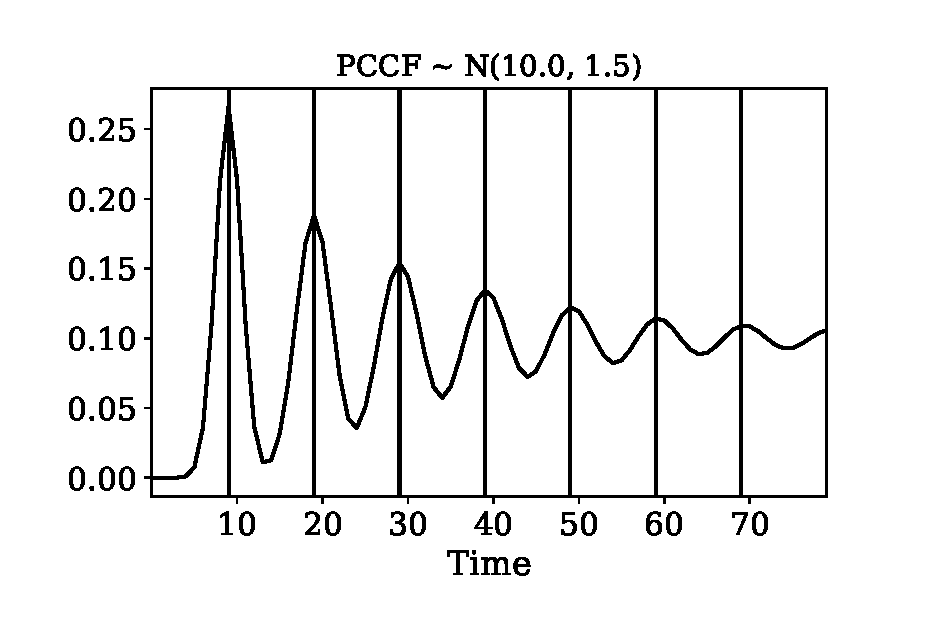
\includegraphics[scale=0.5]{img/pccf_example.eps}
%	\caption{
%		Gaussian PCCF.
%		The oscillating curve depicts probability estimation for the changepoint to occur at corresponding time moment.
%		Peaks are located at time moments $(\mu, 2 \mu, 3\mu, \dots)$.
%	}
%	\label{fig:pccf_example}
%\end{figure}
% Since Pccf decreases its values while oscillating and converging to the constant value over time we effectively choose first $k$ peaks of Pccf by applying threshold.
%By observing how fast Pccf converges to the constant level we can select $k$ based on visual inspection of Pccf behavior.
%Then we would need to select how many change points we need to predict
%After that ROI intervals can be allocated around Pccf's local extremums
\begin{figure}[!htb]
	\centering
	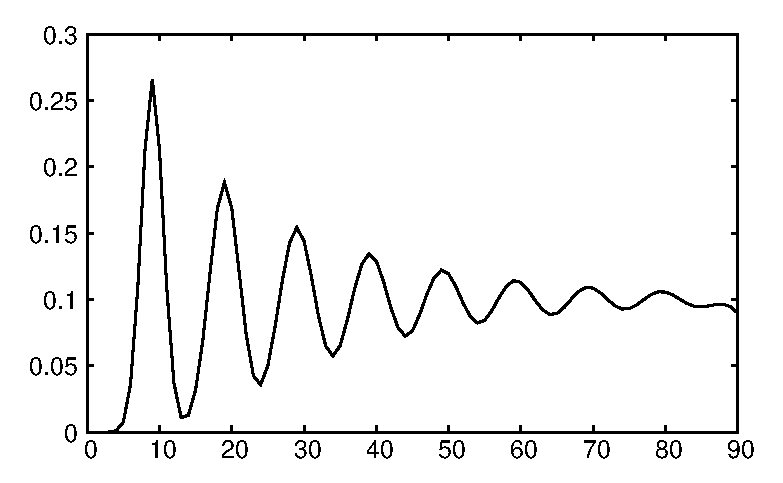
\includegraphics[width=0.7\textwidth]{images/example_pccf.eps}
	\caption{Pccf example}\label{fig:pccf_example}
\end{figure}



\section{Integration with Bayesian detector}
\section{Integration with CuSum}

\chapter{MISC}
External~\cite{shewhart1931economic}
Included article~\cite{sha1}.
Concept drift and change detection problem.
Concept drift can be reduced to change detection in univariate time series?


\begin{itemize}
  \item Change detection:~\cite{basseville1993detection}
  \item Sequential change detection problem is a well studied problem, see for example in~\cite{tartakovsky2014sequential},~\cite{plasse2021streaming}.

  \item Optimality of the change detection procedure was investigated in~\cite{Page1954},~\cite{Shiryaev2010,Shiryaev1961,Shiryaev1963}.
  Asymptotic and nonasymptotic optimality of cumulative sum algorithms was provedin~\cite{lorden1971procedures},~\cite{moustakides1986optimal},~\cite{moustakides2004optimality},~\cite{ritov1990decision}. In~\cite{Shiryaev1963,shiryaev2007optimal} the change point is modelled as a random variable with a known geometric distribution~\cite{veeravalli2014quickest} and optimal algorithm minimizing the average detection delay given constraint on the probability of false alarm is proposed. In our work we minimize the detection delay given a constraint on the maximum delay imposed by the prediction interval width. In~\cite{lorden1971procedures} asymptotic optimality of Cusum~\cite{Page1954} is proved according to the minimax criterion for delay with the mean time between false alarms going to infinity.

  \item Concept drift:
\end{itemize}

\chapter{Conclusion}

\tailmatter
\finnishsummary
Foo bar
%\inputencoding{utf8}
\bibliographystyle{apalike}
\bibliography{references}
\appendices
\appendix{A}
\section{foobar}

\backmatter

\includedarticles
\begin{article}{sha1}
	\arttitle{Modelling Recurrent Events for Improving Online Change Detection}
	\artauthor{Alexandr Maslov, Mykola Pechenizkiy, Indr{\.e} {\v{Z}}liobait{\.e}, and Tommi K\"{a}rkk\"{a}inen}
	\artpublish{Proceedings of the 2016 SIAM International Conference on Data Mining}
	\artyear{2016}
	\artcopyright{XX}
	\artpages{1}
\end{article}

\begin{article}{sha2}
	\arthide
	\arttitle{BLPA: Bayesian learn-predict-adjust method for online detection of recurrent changepoints}
	\artauthor{Alexandr  Maslov, Mykola Pechenizkiy, Yulong  Pei, Indre {\v{Z}}liobait{\.e},  Alexander Shklyaev, Tommi Karkk{\"a}inen, and Hollm{\'e}n, Jaakko}
	\artpublish{2017 International Joint Conference on Neural Networks (IJCNN)}
	\artyear{2017}
	\artcopyright{XXX}
\end{article}
\printindex
\end{document}
